\chapter{NEOIDL: LINGUAGEM PARA ESPECIFICAÇÃO DE CONTRATOS REST	}
\vspace{-6mm}


\section{APRESENTAÇÃO}
\label{apresentacaoNeoIDL}

A \neoidl{} é uma linguagem específica de domínio (\textit{Domain Specific
Language - DSL}) elaborada com o objetivo de possibilitar, em um processo
simples, a elaboração de contratos para serviços REST. Em seu projeto, 
foram considerados os requisitos de concisão, facilidade de compreensão humana,
extensibilidade e suporte à herança simples dos tipos de dados definidos pelo
usuário.

Além de ser uma linguagem, a \neoidl{} é também um \textit{framework} de geração
de código que permite, a partir de contratos especificados na própria
linguagem, a produção da implementação da estrutura do serviço. Os serviços
podem ser construídos em várias linguagens e tecnologias, por meio
de \textit{plugins} da \neoidl{}, conforme será apresentado neste capítulo.

As próximas subseções apresentam o histórico da \neoidl{}, exemplificam sua
sintaxe e descrevem sucintamente seu \textit{framework} de geração de código.


\subsection{Histórico e motivação}
\label{histMotivNeoIDL}
\vspace{-6mm}

A \neoidl{} surgiu no contexto de um acordo de colaboração entre a Universidade
de Brasília e o Exército Brasileiro. O projeto do exército caracterizava-se
pelos requisitos de modularidade -- com a lógica distribuída inclusive
geograficamente -- e de execução em plataformas diversificadas. Diante dessa
necessidade, o Exército desenvolveu um \textit{framework} proprietário,
voltado para arquitetura orientada a serviço e com suporte
a implantação de serviços REST em várias linguagens, denominado \neocortex{}.

A particularidade do \neocortex{} de se utilizar serviços implementados em
várias linguagens motivou o desenvolvimento de um programa gerador de serviços
poliglotas -- que produz código de várias linguagens de programação -- a partir da
descrição do contrato do serviço. A \neoidl{} foi concebida para atender a essa
finalidade. A primeira decisão de projeto da \neoidl{} foi a escolha da
linguagem para se especificar o contrato de serviço.

Porém, as linguagens de programação disponíveis para especificação de
contratos REST, como Swagger\cite{swaggerSite}, WADL\cite{hadley2006web} e
RAML\cite{RAML}, possuiam (e ainda possuem) limitações importantes para a
abordagem desejada, qual seja elaborar primeiramente o contrato e, a
partir dele, gerar a implementação do serviço. Todas essas linguagens utilizam
notações de propósito geral (XML\cite{XML}, JSON\cite{JSon}, YAML\cite{YAML}),
tornando os contratos extensos e de difícil compreensão humana. Além disso,
elas não possuem mecanismos semânticos de extensibilidade e modularidade.

% Problema com a formatação
% \vspace{6mm}
% 
% \begin{figure}[h]
% \begin{small}
% \lstinputlisting[language=JSON,firstnumber=1]{trechos_codigo/exemploSwagger.tex}
% \vspace{-.5cm}
% \end{small}
% \caption{Exemplo de descrição de Web Service em Swagger e YAML}
% \label{lst:exemploSwagger}
% \end{figure}


Partiu-se então para a criação uma nova linguagem, com sintaxe
inspirada em linguagens mais claras e concisas -- como \emph{CORBA
IDL}\texttrademark \cite{corba} e \emph{Apache
Thrift}\texttrademark\cite{thrift} --, e que permitisse ainda a declaração de
tipos de dados definidos pelo usuário e extensibilidade. Ambas, \emph{CORBA} e
\emph{Apache Thrift}, possuem limitações nesses últimos aspectos. A sintaxe e as
características da linguagem \neoidl{} são brevemente discutidas na Subseção
\ref{linguagemNeoIDL}.

Em relação à geração de código, para se viabilizar a geração poliglota de
código, a \neoidl{} foi projetada para possuir uma arquitetura modular, de modo
que novas linguagens ou características de implementação pudessem ser
incorporadas por meio de \textit{plugins} da \neoidl{}. Assim, é possível desenvolver um novo \textit{plugin} para geração de serviços em outras
linguagens, por exemplo PHP, sem alterar qualquer outro componente do \framework,
conforme apresentado na Subseção \ref{frameNeoIDL}.

A primeira versão da \neoidl{}, ponto de onde partiu este trabalho de mestrado,
dava suporte à geração de código em Java, Python e Swagger com as
características necessárias para execução no \neocortex{}. Nessa versão, foram
desenvolvidos para o Exército Brasileiro nove serviços do domínio de Comando e
Controle \cite{david:commandControl}, os quais compreenderam aproximadamente
cinquenta módulos\footnote{O conjunto de documentos
utilizados para descrever contratos na \neoidl{} são denominados
\texttt{módulos}.} e geração de três mil linhas de código Python a partir
da especificação dos contrato em \neoidl{}. Alguns outros serviços foram
ainda implementados em Java.



\subsection{Linguagem}
\label{linguagemNeoIDL}
\vspace{-6mm}

A linguagem \neoidl{} simplifica a especificação de contratos REST pois possui
uma sintaxe concisa, própria de linguagens de especificação de interfaces
(\emph{interface description languages}). Ademais, a \neoidl{} provê mecanismos de
modularização e herança, de forma que os contratos possam ser separados em
módulos, facilitando a herança e manutenção dos
contratos. 

Para demonstrar como os módulos são estruturados na
\neoidl{} e as colaborações da pesquisa para a linguagem, nesta dissertação os
trachos de código \neoidl{} são ilustrados considerando um serviço
hipotético de reserva de livros. Em linhas gerais, o aluno submete um pedido de reserva e, caso todas as condições
sejam satisfeitas, um código de reserva é gerado pelo serviço.

Na primeira parte, um módulo faz uma definição de
tipo de dado (Figura \ref{lst:livrodata-neo}); em seguida, um segundo módulo,
voltado para especificação do serviço em si, importa as definições do primeiro para então declarar as operações do
serviço (Figura \ref{lst:reservalivro-neo}). Por fim, ao módulo de serviço é acrescentada
uma anotação como forma de estender as características da operação (Figura
\ref{lst:annotationNeoIDL}).


\vspace{6mm}

\begin{figure}[h]
\begin{small}
%\lstinputlisting[language=NeoIDL,firstnumber=1]{trechos_codigo/mensagemData.tex}
\lstinputlisting[language=NeoIDL,firstnumber=1]{trechos_codigo/livroData.tex}
\vspace{-.5cm}
\end{small} 
\caption{Tipo de dado Livro definido em \neoidl}
\label{lst:livrodata-neo}
\end{figure}

O trecho ilustrado na Figura \ref{lst:livrodata-neo} faz a definição de
dois tipos de dados. \emph{SituacaoLivro}, declarado no linha 2, é uma estrutura
simples do tipo enumeração. No exemplo, \emph{SituacaoLivro} pode ter os valores
\emph{Bloqueado}, \emph{Reservado} e \emph{Disponivel}.
O outro tipo é \emph{Livro}, declarado entre as linhas 4 e 10,
composto de cinco atributos (\emph{codigo, ISBN, titulo, autor} e
\emph{situacao}).
O atributo \emph{situacao} de \emph{Livro} é do tipo \emph{SituacaoLivro} recém
declarado (linha 2).

Na \neoidl{}, é utilizada a abordagem \emph{convenção sobre configuração}, de
modo que todos os atributos declarados são obrigatórios, a menos que
seja explicitamente declarado diferente. Os atributos \emph{ISBN} e
\emph{autor} do tipo \emph{Livro} são exemplos de atributos opcionais (indicado
pelo símbolo de igual seguido de zero).

Definido o tipo de dado, na linha proposta pela \neoidl{} para
suporte a herança e reuso, o módulo seguinte -- conforme apresentado na Figura
\ref{lst:reservalivro-neo} -- importa o conjunto de definições de
\emph{Livro} e declara a entidade \emph{Reserva} (linha 7) e o serviço
\emph{reservaLivro} (linha 14).
Esse serviço possui duas capacidades:
\emph{solicitaReserva} e \emph{listaReservas}.
A capacidade \emph{solicitaReserva} (linha 16) utiliza a operação \method{post}
para submeter um pedido de reserva (utilizando os tipos \emph{Aluno} e
\emph{Livro}).
A capacidade \emph{listaReservas} (linha 17) tem a finalidade de listar as reservas de um
determinado aluno, por meio da operação
\method{get}.

A instrução \emph{path} (linha 15) completa a especificação do serviço,
indicando o caminho (URI) onde as operações serão disponibilizadas. Esse atribuito é importante para se definir
como as requisições serão roteadas entre os serviços.

\vspace{6mm}

\begin{figure}[htb]
\begin{small}
%\lstinputlisting[language=NeoIDL,firstnumber=1]{trechos_codigo/mensagem.tex}
\lstinputlisting[language=NeoIDL,firstnumber=1]{trechos_codigo/reservaLivro.tex}
\end{small}
\caption{Especificação do serviço de reserva de livros em \neoidl}
\label{lst:reservalivro-neo}
\end{figure}

Seguindo a filosofia de \emph{convenção sobre configuração}, a \neoidl{} assume
que os argumentos das operações dos tipos \method{POST} e \method{PUT} são
enviadas no corpo da requisição. Nas operações dos tipos \method{GET} e
\method{DELETE}, por outro lado, presume-se que os argumentos estão contidos no
\emph{path} da requisição ou ainda como \textit{query string}.

A especificação dos contratos na \neoidl{} pode ser enriquecida de forma simples
com o uso de anotações, pois elas possibilitam estender a semântica
de uma especificação sem que seja necessário alterar a sintaxe da
linguagem \neoidl{}. Essa versatilidade das anotações é bastante útil, pois a
alteração da sintaxe da própria \neoidl{} não é um esfoço trivial, por demandar
a compatibilização de todos os \textit{plugins} já construídos.

O módulo apresentado na Figura \ref{lst:annotationNeoIDL} contém, além das
informações contidas no módulo da Figura \ref{lst:reservalivro-neo}, uma anotação
denominada \emph{SecurityPolicy} (linha 6) que é aplicada ao serviço
\emph{reservaLivro}.
A declaração da anotação é feita ao final do módulo (linhas 14 a 17).

\vspace{6mm}
 
\begin{figure}[htb]
\begin{small}
%\lstinputlisting[language=NeoIDL,firstnumber=1]{trechos_codigo/messageSendAnnotation.tex}
\lstinputlisting[language=NeoIDL,firstnumber=1]{trechos_codigo/reservaLivroAnotacao.tex}
\vspace{-.5cm}
\end{small}
\caption{Especificação de anotação na \neoidl{}}
\label{lst:annotationNeoIDL}
\end{figure}

\begin{figure*}[htb]
\begin{center}
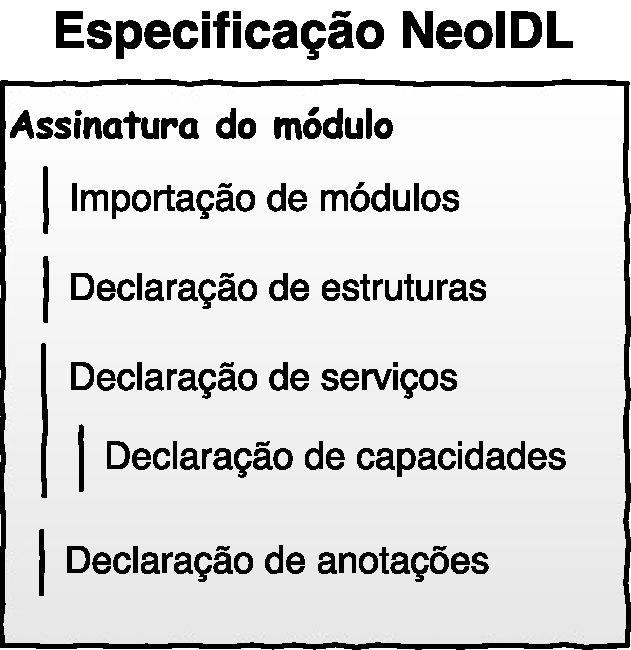
\includegraphics[width=60mm,trim=0cm 0cm 0cm
0cm]{img/NeoIDLModuleSpecificationPt.pdf}
\end{center}
\caption{Estrutura de um módulo \neoidl{}}
\label{fig:moduloNeoIDL}
\end{figure*}

Além de serem aplicáveis a \texttt{resources}, as anotações também podem ser
utilizadas em outros construtores da linguagem: \texttt{module},
\texttt{enum}, \texttt{entity}. Qualquer anotação na \neoidl{} possui a mesma estrutura: um
nome, um elemento alvo e uma lista de propriedades. Todas estas informações
ficam disponíveis para utilização pelos \textit{plugins}.


A estrutura de um módulo \neoidl{}, como pôde ser verificado nesta subseção e
ilustrada na Figura \ref{fig:moduloNeoIDL}, é composta pelas seguintes seções: assinatura do módulo, seção de importação, enumerações e estruturas,
serviços e anotações. O apêndice \ref{apend:estruturaLexicaNeoIDL} apresenta a
estrutura sintática e léxica da \neoidl{} antes de terem sido incorporadas as construções
relativas a \designbycontract{}.



\subsection{\textit{Framework}}
\label{frameNeoIDL}
\vspace{-6mm}

A parte da \neoidl{} responsável pela geração de código de
serviço para as várias linguagens é denominado \framework{} \neoidl{}. O
\framework{} \neoidl{} possui suas partes: o núcleo e os \textit{plugins},
conforme ilustrado na Figura \ref{fig:programGenerator}.
O núcleo é composto de módulos responsáveis (a) por fazer o \textit{parse}\footnote{O \textit{parser} da \neoidl{}
foi construído utilizando \bnfc{} \cite{ranta-bnfc:2012} com a linguagem de
programação funcional Haskell.}
do contrato escrito em \neoidl{}, (b) por processar a sintaxe da linguagem \neoidl{} e (c) pelo gerenciamento dos \textit{plugins}.

\begin{figure*}[h]
\begin{center}
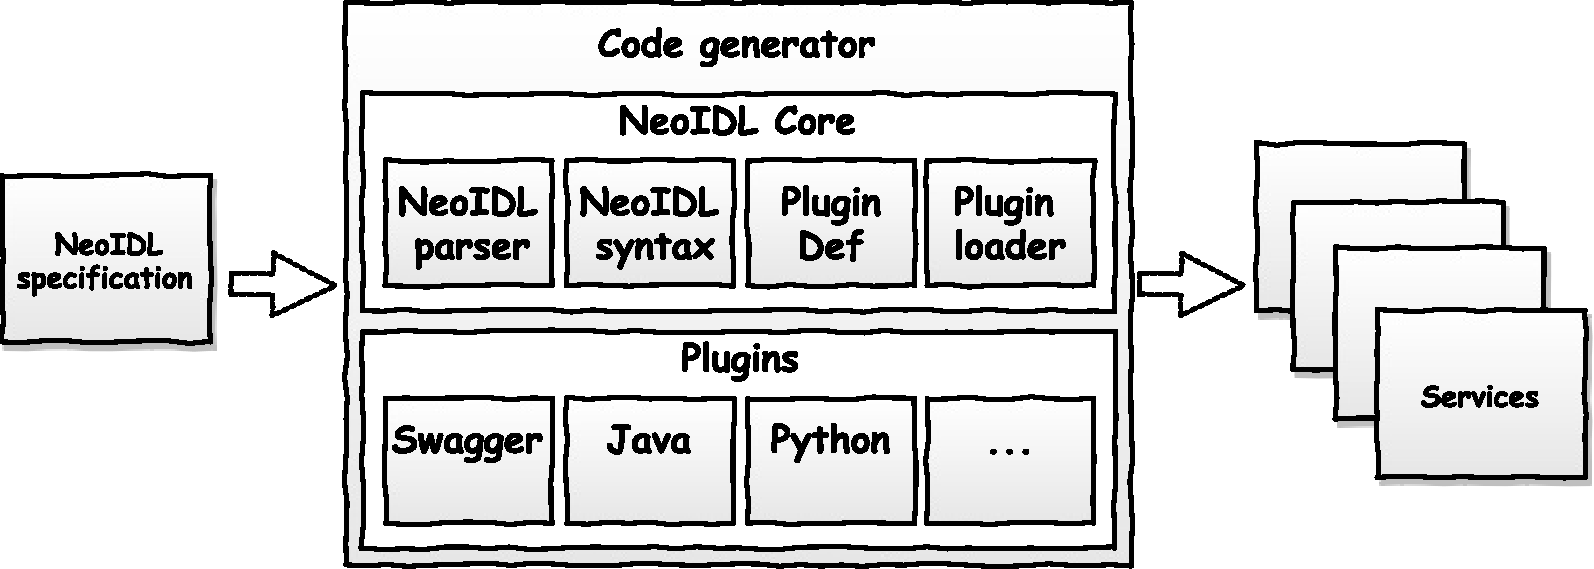
\includegraphics[width=120mm,trim=0cm 0cm 0cm
0cm]{img/NeoIDLCodeGenerator.pdf}
\vspace{-.5cm}
\end{center}
\caption{Gerador de código da \neoidl{}}
\label{fig:programGenerator}
\end{figure*}

Fora do núcleo da \neoidl{} ficam os \textit{plugins}, responsáveis,
cada um, por gerar código para as linguagens de destino. Assim, para se
possibilitar a geração de código para uma nova linguagem ou segundo uma nova arquitetura, um
novo \textit{plugin} deve ser desenvolvido. A primeira versão da \neoidl{}
possuia \textit{plugins} para Python, Java e Swagger.

As próximas subseções resumem o funcionamento de
dois módulos onde estão contidas os principais trechos da lógica implementada na \neoidl{}: O
\textit{PluginDef} e \textit{PluginLoader}. Mais detalhes podem ser obtidos na
publicação \textit{NeoIDL: A Domain Specific Language for Specifying REST
Contracts Detailed Design and Extended Evaluation} \cite{lima2015neoidl}.
 

\subsubsection{Componente PluginDef}{\label{sec:plugindef}}

O módulo \texttt{PluginDef} estabelece as definições de regras de projeto
(\textit{Design Rules}) obrigatórias para o desenvolvimento de
\textit{plugins}, padronizando-os. De acordo com as regras de projeto, cada
\textit{plugin} precisa declarar uma instância do tipo \emph{Plugin} e implementar uma função de
transformação de acordo com a assinatura definida.

Além disso, cada instância de  
\texttt{Plugin} precisa ter o nome do \texttt{plugin} de forma que o
componenente \texttt{PluginLoader} (Subseção \ref{compPluginLoader}) possa obter
os dados necessários para o seu processamento.
Resumidamente, a execução de um \textit{plugin} consiste em aplicar sua função
de transformação a um módulo \neoidl{} e produzir uma lista de
arquivos de código fonte. 


\subsubsection{Componente PluginLoader}
\label{compPluginLoader}

O carregamento e validação dos \textit{plugins} são competências do componente
\texttt{PluginLoader}. Se todas as regras de definição do \textit{plugin}
tiverem sido atendidas, o \textit{plugin} é carregado e estará pronto para ser
 acionado. Caso contrário, algumas exceções podem ocorrer, como, por exemplo, não haver definição de
nenhum \textit{plugin} no arquivo:
\vspace{-6mm}

\begin{tabbing}\tt
~\char36{}\char46{}\char47{}neoIDL\\
\tt
~neoIDL\char58{}~panic\char33{}~\char40{}the~\char96{}impossible\char39{}~happened\char41{}\\
\tt ~~\char40{}GHC~version~7\char46{}6\char46{}3~for~x86\char95{}64\char45{}darwin\char41{}\char58{}\\
\tt ~~~~Not~in~scope\char58{}~\char96{}Plugins\char46{}Python\char46{}plugin\char39{}
\end{tabbing}
\vspace{-6mm}

Ou ainda em razão de o \textit{plugin} não ser uma instância do tipo
\texttt{Plugin}:

\vspace{-6mm}
\begin{tabbing}\tt
~\char36{}\char46{}\char47{}neoIDL\\
\tt
~neoIDL\char58{}~panic\char33{}~\char40{}the~\char96{}impossible\char39{}~happened\char41{}\\
\tt ~\char40{}GHC~version~7\char46{}6\char46{}3~for~x86\char95{}64\char45{}darwin\char41{}\char58{}\\
\tt ~~Couldn\char39{}t~match~expected~type~\char96{}Plugin\char39{}\\
\tt ~~~with~actual~type~\char96{}\char91{}GHC\char46{}Types\char46{}Char\char93{}\char39{}
\end{tabbing}


\section{AVALIAÇÃO EMPÍRICA}
\label{EstudoExpressividadeReuso}
\vspace{-6mm}

A primeira versão da \neoidl{} foi submetida a um estudo empírico de sua expressividade 
e reuso em um contexto real. As próximas subseções apresentam 
o resultado da análise comparativa da representação de 44 (quarenta e quatro)
contratos escritos em Swagger v1.2 em relação à mesma especificação em
\neoidl{}.

Esse estudo é uma das contribuições deste trabalho de mestrado e foi publicado
no periódico IJSeke \cite{lima2015neoidl}.

\subsection{Expressividade}
\label{estudoExpressividadeNeoIDL}
\vspace{-6mm}

A \neoidl{} é uma DSL, conforme apresentado na Seção \ref{apresentacaoNeoIDL},
e como tal se destina a atender a um propósito específico, nem mais, nem menos
\cite{hudak1998modular}. A \neoidl{} foi projetada para permitir a
especificação de contratos de serviços REST de forma mais expressiva e concisa,
facilitando-se a escrita e leitura por humanos (mais detalhes na Subseção
\ref{histMotivNeoIDL}).

Programas escritos em DSLs costumam ser mais fáceis de escrever e,
consequentemente, mais fáceis de se manter comparavelmente a programas escritos
em linguagens de propósito geral \cite{hudak1998modular}. Isso se deve
justamente ao fato de a DSL tratar apenas um conjunto reduzido de situações e
problemas, fazendo com que ela seja, muitas vezes, mais acessível ao público
geral \cite{taha2008domain}.

A expressividade é um dos principais critérios para se escolher uma
linguagem. Entretanto a linguagem que não expressa todas as situações
necessárias ao seu contexto de uso, por óbvio, não pode ser usada
\cite{mackinlay1985expressiveness}. Nesse sentido, o primeiro teste a que a
\neoidl{} foi submetida constituiu-se na produção de contratos e serviços reais
no início do projeto com o Exército Brasileiro (vide Subseção \ref{histMotivNeoIDL}).

Assim, tendo a \neoidl{} demonstrado sua capacidade de representar contratos
REST reais, foi realizada uma segunda análise: quão expressiva seria a
\neoidl{} em comparação com outra linguagem com o mesmo objetivo. Foi escolhida
Swagger \cite{swaggerSite}, uma linguagem de especificação de contratos REST
cujo uso tem crescido pela indústria.
Em Swagger, os contratos são escritos em JSON\cite{JSon} ou YAML\cite{YAML},
ambos com uma estrutura geral de chave-valor.

Sendo a facilidade de compreensão e manipulação por humanos um dos pilares
de desenvolvimento da \neoidl{}, foi adotado o critério de comparar
a expressividade em termos de quantidade de linhas de código (SLOC - do inglês
\textit{Source Lines of Code}), uma vez que muitas linhas significam maior
esforço para escrita, sobretudo na abordagem \CtFirst{}.

Com esse propósito, foi obtido um conjunto de 44 contratos do Exército
Brasileiro especificados em Swagger. A primeira etapa foi reescrever esses
contratos em \neoidl{} e então comparar a quantidade de linhas de código
produzida com a quantidade de linhas de código dos contratos originais.

Para a
transcrição dos contratos, em razão da \neoidl{} não possuir recursos para
trans\-crição bidirecional de Swagger para \neoidl{}, foi desenvolvido
e utilizado um \textit{script} na linguagem \textit{Perl}, 
o qual consta do Apêndice \ref{scriptSwagger2NeoIDL} desta dissertação.

Os quarenta e quatro contratos em Swagger contabilizaram 13.921 linhas de
especificação. Os mesmos contratos especificados em \neoidl{} somaram 5.140
linhas de especificação, correspondendo a uma redução média de 63\%. Assim, para
cada 10 linhas de especificação em Swagger são requeridas 4 linhas de
especificação \neoidl{}. Nessa análise foram consideradas linhas físicas de
código, ignorando-se linhas em branco ou compostas apenas de delimitadores.

A proporção de redução não se deu de forma igual em todos os contratos. Por
exemplo, o contrato de um determinado serviço\footnote{Os nomes reais e
conteúdos dos contratos foram omitidos em razão de acordo de confidencialidade.}
requereu 367 linhas na especificação Swagger e 112 linhas na especificação \neoidl{} --
redução da ordem de 69\%.
Em contraponto, outro serviço especificado em Swagger possuia 81 linhas e o
correspondente em \neoidl{} 42 linhas -- redução de linhas de código pouco inferior a 50\%.

Estatisticamente, o tamanho original dos contratos tem apenas uma pequena
influência na expressividade avaliada. Dessa forma, não é possível assumir que
contratos Swagger maiores terão um correspondente proporcionalmente menor em
\neoidl{}.
Outros atributos como documentação mais descritiva, quantidade de entidades e o
número de capacidades de cada serviço também não possuem correlação com redução
de linha de código maior ou menor após o processo de tranformação para
\neoidl{}.

A Tabela \ref{tab:size-corr} apresenta a correlação entre a
melhoria na expressividade observada (medida como percentual de redução após a
transformação da especificação Swagger em especificação \neoidl{}) e algumas
métricas relacionadas ao tamanho da especificação original em Swagger. Na
Correlação Pearson \cite{benesty2009pearson}, um \emph{p-value} igual a 1 significa correlação
positiva perfeita. Um \emph{p-value} igual a -1 significa correlação negativa
perfeita, enquanto \emph{p-value} igual a zero indica que as medidas não possuem
correlação linear.

% 
% 
% Table~\ref{tab:size-corr} presents the correlation between the improvement of
% expressiveness (measured as the percentage of reduction obtained after
% transforming Swagger specifications into \neoidl{} specifications) and some
% metrics related to the size of the original Swagger specifications.

\begin{table}[htb]
\caption{Correlação entre o aumento do grau de expressividade com o tamanho da
especificação em Swagger}
\begin{center} 
\begin{tabular}{lrr} 
\toprule
Métrica & Correlação Pearson's & \emph{p-value} \\ \hline \hline 
LOC da especificação Swagger & 0.19 &  0.20 \\ 
Número de serviços & 0.14 & 0.35 \\ 
Numero de capacidades & 0.14 & 0.34 \\
Número de entidades & 0.20 & 0.18 \\ \bottomrule 
\end{tabular} 
\end{center}
\label{tab:size-corr}
\end{table}



\subsection{Potencial de reuso}

De forma similar à \neoidl{}, Swagger também possui recursos para reuso de
estruturas, por meio de referências (marcação \$ref). Entretanto, esse recurso
praticamente não foi explorado no conjunto de contratos analisados, o que
ocasinou a duplicação da declaração de estruturas entre os diferentes arquivos
de especificação Swagger. Isso se deve, provavelmente, ao modo não intuitivo de
se fazer referência em Swagger (baseado na referência a outro arquivo JSON) e à
dificuldade de se identificar que uma determinada entidade foi declarada em
outro contrato.

No conjunto dos 44 contratos Swagger analisados foram identificadas 42 entidades
especificadas em pelo menos dois contratos. Uma entidade específica, de
identificação da posição geográfica, muito utilizada no domínio de Comando e Controle, aparece
declarada 12 vezes em contratos distintos. A Tabela \ref{estatisticaEntidades}
mostra a estatística de repetição da especificação de contratos.
 
\begin{table}[!bth] 
\centering
\vspace{0.5cm}
\footnotesize
\begin{tabular}{r|r}
Quantidade de & Quantidade de \\
entidades &  especificações \\
\hline   
420 & 1 \\
26 & 2 \\
5 & 3 \\
7 & 4 \\
2 & 5 \\
2 & 6 \\
1 & 10 \\
1 & 12 \\
%\begin{tabular}{|r|r|r|r|r|r|r|r|r|}
%\hline   
%Quantidade de entidades & 420 & 26 & 5 & 7 & 2 & 2 & 1 & 1 \\
%\hline
%Quantidade de especificações & 1 & 2 & 3 & 4 & 5 & 6 & 10 & 12 \\
%\hline

\end{tabular}
\caption{Estatística de entidades declaradas repetidamente entre contratos}
\label{estatisticaEntidades}
\end{table}

Os resultados do estudo sobre a expressividade e potencial de reuso em Swagger
comprovaram, no contexto dos contratos reais avaliados, que a especificação de
contratos REST nessa linguagem carece de melhorias importantes. Verificou-se,
ainda, que a \neoidl{} é mais concisa e expressiva que Swagger para representar
as mesmas informações de contratos REST. Sob a ótica do reuso, a abordagem proposta pela
\neoidl{}, baseada em importações de especificações de entidades, tende a
contribuir para a identificação de entidades já declaradas, facilitando que
elas sejam reusadas.

Este capítulo tratou de como foi concebida e como estava estruturada a
\neoidl{} antes da incorporações de construções de \designbycontract{}. Em
outras palavras, apresentou-se o alicerce sobre o qual foram
desenvolvidas a extensão da linguagem e o \framework{} \neoidl{} com suporte a
contratos com garantias típicas de \designbycontract{}, contribuições que serão
detalhadamente descritas no próximo capítulo.
